% Options for packages loaded elsewhere
\PassOptionsToPackage{unicode}{hyperref}
\PassOptionsToPackage{hyphens}{url}
\PassOptionsToPackage{dvipsnames,svgnames,x11names}{xcolor}
%
\documentclass[
  letterpaper,
  DIV=11,
  numbers=noendperiod]{scrartcl}

\usepackage{amsmath,amssymb}
\usepackage{iftex}
\ifPDFTeX
  \usepackage[T1]{fontenc}
  \usepackage[utf8]{inputenc}
  \usepackage{textcomp} % provide euro and other symbols
\else % if luatex or xetex
  \usepackage{unicode-math}
  \defaultfontfeatures{Scale=MatchLowercase}
  \defaultfontfeatures[\rmfamily]{Ligatures=TeX,Scale=1}
\fi
\usepackage{lmodern}
\ifPDFTeX\else  
    % xetex/luatex font selection
\fi
% Use upquote if available, for straight quotes in verbatim environments
\IfFileExists{upquote.sty}{\usepackage{upquote}}{}
\IfFileExists{microtype.sty}{% use microtype if available
  \usepackage[]{microtype}
  \UseMicrotypeSet[protrusion]{basicmath} % disable protrusion for tt fonts
}{}
\makeatletter
\@ifundefined{KOMAClassName}{% if non-KOMA class
  \IfFileExists{parskip.sty}{%
    \usepackage{parskip}
  }{% else
    \setlength{\parindent}{0pt}
    \setlength{\parskip}{6pt plus 2pt minus 1pt}}
}{% if KOMA class
  \KOMAoptions{parskip=half}}
\makeatother
\usepackage{xcolor}
\setlength{\emergencystretch}{3em} % prevent overfull lines
\setcounter{secnumdepth}{-\maxdimen} % remove section numbering
% Make \paragraph and \subparagraph free-standing
\makeatletter
\ifx\paragraph\undefined\else
  \let\oldparagraph\paragraph
  \renewcommand{\paragraph}{
    \@ifstar
      \xxxParagraphStar
      \xxxParagraphNoStar
  }
  \newcommand{\xxxParagraphStar}[1]{\oldparagraph*{#1}\mbox{}}
  \newcommand{\xxxParagraphNoStar}[1]{\oldparagraph{#1}\mbox{}}
\fi
\ifx\subparagraph\undefined\else
  \let\oldsubparagraph\subparagraph
  \renewcommand{\subparagraph}{
    \@ifstar
      \xxxSubParagraphStar
      \xxxSubParagraphNoStar
  }
  \newcommand{\xxxSubParagraphStar}[1]{\oldsubparagraph*{#1}\mbox{}}
  \newcommand{\xxxSubParagraphNoStar}[1]{\oldsubparagraph{#1}\mbox{}}
\fi
\makeatother


\providecommand{\tightlist}{%
  \setlength{\itemsep}{0pt}\setlength{\parskip}{0pt}}\usepackage{longtable,booktabs,array}
\usepackage{calc} % for calculating minipage widths
% Correct order of tables after \paragraph or \subparagraph
\usepackage{etoolbox}
\makeatletter
\patchcmd\longtable{\par}{\if@noskipsec\mbox{}\fi\par}{}{}
\makeatother
% Allow footnotes in longtable head/foot
\IfFileExists{footnotehyper.sty}{\usepackage{footnotehyper}}{\usepackage{footnote}}
\makesavenoteenv{longtable}
\usepackage{graphicx}
\makeatletter
\def\maxwidth{\ifdim\Gin@nat@width>\linewidth\linewidth\else\Gin@nat@width\fi}
\def\maxheight{\ifdim\Gin@nat@height>\textheight\textheight\else\Gin@nat@height\fi}
\makeatother
% Scale images if necessary, so that they will not overflow the page
% margins by default, and it is still possible to overwrite the defaults
% using explicit options in \includegraphics[width, height, ...]{}
\setkeys{Gin}{width=\maxwidth,height=\maxheight,keepaspectratio}
% Set default figure placement to htbp
\makeatletter
\def\fps@figure{htbp}
\makeatother
% definitions for citeproc citations
\NewDocumentCommand\citeproctext{}{}
\NewDocumentCommand\citeproc{mm}{%
  \begingroup\def\citeproctext{#2}\cite{#1}\endgroup}
\makeatletter
 % allow citations to break across lines
 \let\@cite@ofmt\@firstofone
 % avoid brackets around text for \cite:
 \def\@biblabel#1{}
 \def\@cite#1#2{{#1\if@tempswa , #2\fi}}
\makeatother
\newlength{\cslhangindent}
\setlength{\cslhangindent}{1.5em}
\newlength{\csllabelwidth}
\setlength{\csllabelwidth}{3em}
\newenvironment{CSLReferences}[2] % #1 hanging-indent, #2 entry-spacing
 {\begin{list}{}{%
  \setlength{\itemindent}{0pt}
  \setlength{\leftmargin}{0pt}
  \setlength{\parsep}{0pt}
  % turn on hanging indent if param 1 is 1
  \ifodd #1
   \setlength{\leftmargin}{\cslhangindent}
   \setlength{\itemindent}{-1\cslhangindent}
  \fi
  % set entry spacing
  \setlength{\itemsep}{#2\baselineskip}}}
 {\end{list}}
\usepackage{calc}
\newcommand{\CSLBlock}[1]{\hfill\break\parbox[t]{\linewidth}{\strut\ignorespaces#1\strut}}
\newcommand{\CSLLeftMargin}[1]{\parbox[t]{\csllabelwidth}{\strut#1\strut}}
\newcommand{\CSLRightInline}[1]{\parbox[t]{\linewidth - \csllabelwidth}{\strut#1\strut}}
\newcommand{\CSLIndent}[1]{\hspace{\cslhangindent}#1}

\usepackage{booktabs}
\usepackage{longtable}
\usepackage{array}
\usepackage{multirow}
\usepackage{wrapfig}
\usepackage{float}
\usepackage{colortbl}
\usepackage{pdflscape}
\usepackage{tabu}
\usepackage{threeparttable}
\usepackage{threeparttablex}
\usepackage[normalem]{ulem}
\usepackage{makecell}
\usepackage{xcolor}
\KOMAoption{captions}{tableheading}
\makeatletter
\@ifpackageloaded{caption}{}{\usepackage{caption}}
\AtBeginDocument{%
\ifdefined\contentsname
  \renewcommand*\contentsname{Table of contents}
\else
  \newcommand\contentsname{Table of contents}
\fi
\ifdefined\listfigurename
  \renewcommand*\listfigurename{List of Figures}
\else
  \newcommand\listfigurename{List of Figures}
\fi
\ifdefined\listtablename
  \renewcommand*\listtablename{List of Tables}
\else
  \newcommand\listtablename{List of Tables}
\fi
\ifdefined\figurename
  \renewcommand*\figurename{Figure}
\else
  \newcommand\figurename{Figure}
\fi
\ifdefined\tablename
  \renewcommand*\tablename{Table}
\else
  \newcommand\tablename{Table}
\fi
}
\@ifpackageloaded{float}{}{\usepackage{float}}
\floatstyle{ruled}
\@ifundefined{c@chapter}{\newfloat{codelisting}{h}{lop}}{\newfloat{codelisting}{h}{lop}[chapter]}
\floatname{codelisting}{Listing}
\newcommand*\listoflistings{\listof{codelisting}{List of Listings}}
\makeatother
\makeatletter
\makeatother
\makeatletter
\@ifpackageloaded{caption}{}{\usepackage{caption}}
\@ifpackageloaded{subcaption}{}{\usepackage{subcaption}}
\makeatother

\ifLuaTeX
  \usepackage{selnolig}  % disable illegal ligatures
\fi
\usepackage{bookmark}

\IfFileExists{xurl.sty}{\usepackage{xurl}}{} % add URL line breaks if available
\urlstyle{same} % disable monospaced font for URLs
\hypersetup{
  pdftitle={HW6},
  pdfauthor={Maiko Hata and Michelle Cui},
  colorlinks=true,
  linkcolor={blue},
  filecolor={Maroon},
  citecolor={Blue},
  urlcolor={Blue},
  pdfcreator={LaTeX via pandoc}}


\title{HW6}
\author{Maiko Hata and Michelle Cui}
\date{2024-11-06}

\begin{document}
\maketitle


\section{\textless\textless\textless\textless\textless\textless\textless{}
Updated upstream}\label{updated-upstream}

\begin{quote}
\begin{quote}
\begin{quote}
\begin{quote}
\begin{quote}
\begin{quote}
\begin{quote}
Stashed changes
\end{quote}
\end{quote}
\end{quote}
\end{quote}
\end{quote}
\end{quote}
\end{quote}

\section{What is Intersectionality and why is it
important?}\label{what-is-intersectionality-and-why-is-it-important}

Crenshaw (1987) emphasized the importance of intersectionality as a
research framework, stating that ``Because the intersectional experience
is greater than the sum of racism and sexism, any analysis that does not
take intersectionality into account cannot sufficiently address the
particular manner in which Black women are subordinated'' (p.~140).''
Studies show that this stands true as studies show that infants and
toddlers of color are underrepresented in Early Intervention (EI)
services (see Cycyk et al. 2022; Cho and Gannotti 2005; Cycyk and Durán
2020).

\section{Table 1}\label{table-1}

\begin{longtable}[]{@{}llrrrr@{}}
\toprule\noalign{}
sex & frl & math\_mean & math\_sd & rdg\_mean & rdg\_sd \\
\midrule\noalign{}
\endhead
\bottomrule\noalign{}
\endlastfoot
boy & no & 492.85 & 46.34 & 441.46 & 32.32 \\
boy & yes & 469.87 & 46.09 & 425.38 & 26.63 \\
girl & no & 501.21 & 45.96 & 448.54 & 34.52 \\
girl & yes & 477.51 & 46.30 & 430.80 & 27.42 \\
\end{longtable}

Description: As it is presented in the Table 1, both boy and girl in the
no free/reduced lunch group has higher average standardized scores than
the boy and girls in the free lunch group. In addition, in the free
lunch group, the boys average standardized scores is lower than the
girls. It seems the both household income and gender influence the
students reading and math performance.

\section{Plot 1 Relationship between teacher experience and math
scores}\label{plot-1-relationship-between-teacher-experience-and-math-scores}

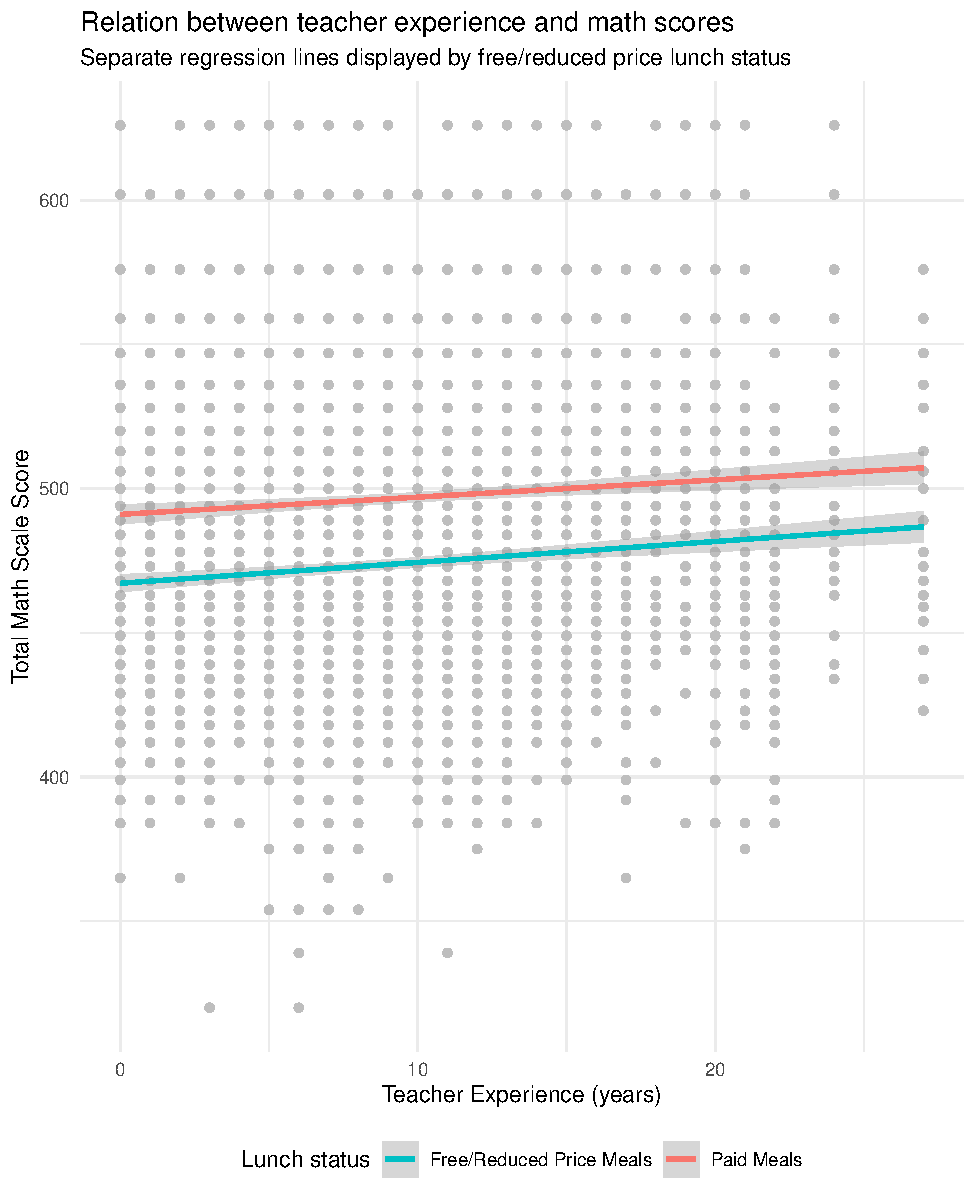
\includegraphics{HW6v2_files/figure-pdf/unnamed-chunk-4-1.pdf}

\newpage

\section*{References}\label{references}
\addcontentsline{toc}{section}{References}

\phantomsection\label{refs}
\begin{CSLReferences}{1}{0}
\bibitem[\citeproctext]{ref-cho2005korean}
Cho, Su-Je, and Mary E Gannotti. 2005. {``Korean-American Mothers'
Perception of Professional Support in Early Intervention and Special
Education Programs.''} \emph{Journal of Policy and Practice in
Intellectual Disabilities} 2 (1): 1--9.

\bibitem[\citeproctext]{ref-crenshaw1987theories}
Crenshaw, Martha. 1987. {``Theories of Terrorism: Instrumental and
Organizational Approaches.''} \emph{The Journal of Strategic Studies} 10
(4): 13--31.

\bibitem[\citeproctext]{ref-cycyk2022moving}
Cycyk, Lauren M, Stephanie De Anda, Katrina L Ramsey, Bruce S Sheppard,
and Katharine Zuckerman. 2022. {``Moving Through the Pipeline: Ethnic
and Linguistic Disparities in Special Education from Birth Through Age
Five.''} \emph{Educational Researcher} 51 (7): 451--64.

\bibitem[\citeproctext]{ref-cycyk2020supporting}
Cycyk, Lauren M, and Lillian Durán. 2020. {``Supporting Young Children
with Disabilities and Their Families from Undocumented Immigrant
Backgrounds: Recommendations for Program Leaders and Practitioners.''}
\emph{Young Exceptional Children} 23 (4): 212--24.

\end{CSLReferences}




\end{document}
